%% ICS 605 Final Presentation — Nicholas Fairhart
\documentclass[aspectratio=169,11pt]{beamer}

%% Theme — Metropolis
\usetheme{metropolis}
\metroset{progressbar=frametitle, block=fill, titleformat=smallcaps}

%% Packages
\usepackage{booktabs}
\usepackage{graphicx}
\usepackage{tikz}
\usetikzlibrary{arrows.meta, shapes.geometric, positioning, fit, backgrounds}
\usepackage{xcolor}
\usepackage{amsmath}

%% Colors — UH Manoa green accent
\definecolor{uhgreen}{RGB}{0,100,55}
\definecolor{accentblue}{RGB}{30,100,200}
\definecolor{warnred}{RGB}{200,40,40}
\definecolor{lightbg}{RGB}{248,248,248}

\setbeamercolor{normal text}{fg=black, bg=white}
\setbeamercolor{frametitle}{bg=uhgreen, fg=white}
\setbeamercolor{title separator}{fg=uhgreen}
\setbeamercolor{progress bar}{fg=uhgreen, bg=uhgreen!25}
\setbeamercolor{alerted text}{fg=warnred}
\setbeamercolor{example text}{fg=accentblue}
\setbeamercolor{block title}{bg=uhgreen!90, fg=white}
\setbeamercolor{block body}{bg=uhgreen!8, fg=black}
\setbeamercolor{block title alerted}{bg=warnred!80, fg=white}
\setbeamercolor{block body alerted}{bg=warnred!8, fg=black}

%% Helpers
\newcommand{\highlight}[1]{\textcolor{accentblue}{\textbf{#1}}}
\newcommand{\warn}[1]{\textcolor{warnred}{#1}}

% ---------------------------------------------------------------
\title[Resume-Job Fit via Fine-Tuning]{Fine-Tuning a Local Language Model\\for Structured Resume-Job Fit Analysis}
\author{Nicholas Fairhart}
\institute{University of Hawaii at Manoa \\ ICS 605 --- Final Project}
\date{May 2026}
% ---------------------------------------------------------------

\begin{document}

% ===============================================================
\maketitle

% ===============================================================
\begin{frame}{The Problem}
\begin{columns}[T]
\begin{column}{0.55\textwidth}
  \small
  \textbf{Job searching is a communication problem.}
  \begin{itemize}
    \setlength\itemsep{0.15em}
    \item Candidates may have the right skills but resumes don't ``speak the language'' of job descriptions
    \item Recruiters review hundreds of applications, often without domain expertise
    \item Especially hard for \alert{career-returners}: legitimate experience, employment gap stigma
  \end{itemize}
  \textbf{Existing tools fall short:}
  \begin{itemize}
    \setlength\itemsep{0.1em}
    \item General-purpose LLM chat gives isolated line feedback
    \item No structured output $\to$ hard to act on
    \item Requires API access / ongoing cost
  \end{itemize}
\end{column}
\begin{column}{0.42\textwidth}
  \small
  \begin{block}{Goal}
    Build a \textbf{structured, actionable} fit analyzer that runs \textbf{entirely on consumer hardware}---no cloud, no recurring cost.
  \end{block}
  \begin{block}{Eight output criteria}
    Match score $\cdot$ Experience level fit $\cdot$
    Matching strengths $\cdot$ Skill gaps $\cdot$
    ATS keyword coverage $\cdot$
    Resume improvements $\cdot$
    Recommended activities
  \end{block}
\end{column}
\end{columns}
\end{frame}

% ===============================================================
\begin{frame}{System Overview}
\begin{center}
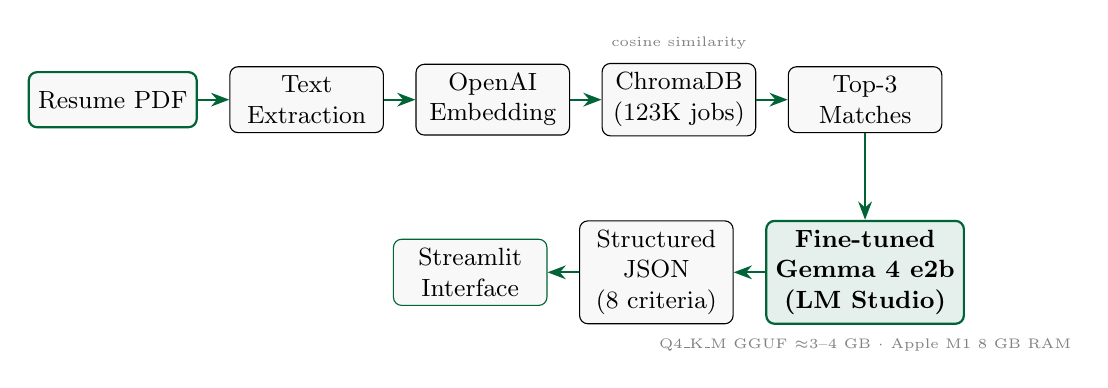
\begin{tikzpicture}[
  node distance=0.55cm and 0.4cm,
  box/.style={draw, rounded corners=3pt, fill=lightbg, minimum height=0.7cm,
              minimum width=1.95cm, align=center, font=\small},
  accent/.style={draw=uhgreen, thick, rounded corners=3pt, fill=uhgreen!10,
                 minimum height=0.7cm, minimum width=1.95cm, align=center, font=\small\bfseries},
  arrow/.style={-Stealth, thick, uhgreen},
  lbl/.style={font=\tiny, text=gray}
]
\node[box, draw=uhgreen, thick] (pdf)   {Resume PDF};
\node[box, right=of pdf]        (parse) {Text\\Extraction};
\node[box, right=of parse]      (embed) {OpenAI\\Embedding};
\node[box, right=of embed]      (chroma){ChromaDB\\(123K jobs)};
\node[box, right=of chroma]     (top3)  {Top-3\\Matches};

\node[accent, below=1.1cm of top3]     (llm)   {Fine-tuned\\Gemma 4 e2b\\(LM Studio)};
\node[box, left=of llm]                (json)  {Structured\\JSON\\(8 criteria)};
\node[box, draw=uhgreen, left=of json] (ui)    {Streamlit\\Interface};

\draw[arrow] (pdf)--(parse); \draw[arrow] (parse)--(embed);
\draw[arrow] (embed)--(chroma); \draw[arrow] (chroma)--(top3);
\draw[arrow] (top3)--(llm);
\draw[arrow] (llm)--(json); \draw[arrow] (json)--(ui);

\node[lbl, below=0.05cm of llm] {Q4\_K\_M GGUF $\approx$3--4 GB $\cdot$ Apple M1 8 GB RAM};
\node[lbl, above=0.05cm of chroma] {cosine similarity};
\end{tikzpicture}
\end{center}
\begin{center}
  \small Fully local inference after training --- \highlight{no API cost}, no internet required at runtime
\end{center}
\end{frame}

% ===============================================================
\begin{frame}{Data}
\begin{columns}[T]
\begin{column}{0.48\textwidth}
  \small
  \textbf{Two public Kaggle datasets}
  \begin{itemize}
    \setlength\itemsep{0.1em}
    \item \textbf{Resumes}: 2,483 across 25 categories (healthcare, engineering, finance, \ldots)
    \item \textbf{Jobs}: 123,849 LinkedIn postings with title, company, experience level, description
  \end{itemize}
  \textbf{Pair construction}
  \begin{itemize}
    \setlength\itemsep{0.1em}
    \item 100 resumes sampled per category (24 categories)
    \item Per resume: \textbf{top-3 semantic matches} via ChromaDB + \textbf{2 random} postings
    \item Random pairs add score variance; stopped at \highlight{10,000 pairs}
  \end{itemize}
\end{column}
\begin{column}{0.48\textwidth}
  \small
  \textbf{Teacher labeling --- GPT-4-nano}
  \begin{itemize}
    \setlength\itemsep{0.1em}
    \item Structured output schema: 8 criteria per pair
    \item $\approx$17M tokens processed
    \item Total cost: \highlight{\$4.68}
    \item Goal: \emph{consistent} scoring behavior, not perfect ground truth
  \end{itemize}
  \begin{block}{Final split}
    \centering\small
    \begin{tabular}{lr}
      Train      & 9,000 pairs \\
      Validation &   997 pairs \\
      \midrule
      Total      & 10,000 pairs \\
    \end{tabular}
  \end{block}
\end{column}
\end{columns}
\end{frame}

% ===============================================================
\begin{frame}{Method --- Knowledge Distillation}
\begin{center}
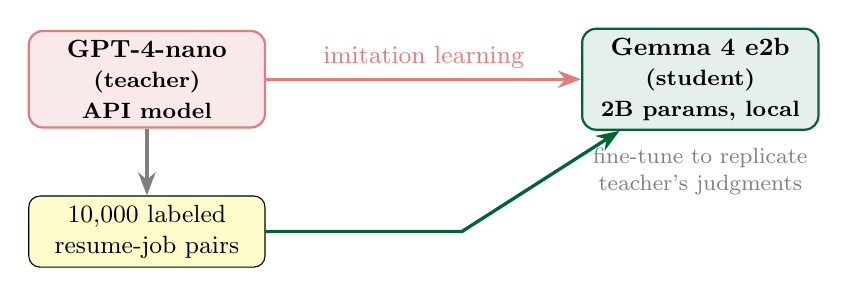
\begin{tikzpicture}[
  node distance=0.9cm and 1.8cm,
  model/.style={draw, thick, rounded corners=5pt, minimum width=3cm,
                minimum height=1.1cm, align=center, font=\small\bfseries},
  arrow/.style={-Stealth, very thick}
]
  \node[model, fill=warnred!10, draw=warnred!60] (teacher)
    {GPT-4-nano\\{\footnotesize (teacher)}\\{\footnotesize API model}};
  \node[model, fill=uhgreen!10, draw=uhgreen, right=4cm of teacher] (student)
    {Gemma 4 e2b\\{\footnotesize (student)}\\{\footnotesize 2B params, local}};
  \node[draw, rounded corners, fill=yellow!20, below=0.85cm of teacher,
        minimum width=3cm, align=center, font=\small] (data)
    {10,000 labeled\\resume-job pairs};

  \draw[arrow, warnred!60] (teacher) -- node[above, font=\small]{imitation learning} (student);
  \draw[arrow, gray]       (teacher) -- (data);
  \draw[arrow, uhgreen]    (data) -- ++(4,0) -- (student);
  \node[below=0.1cm of student, font=\footnotesize, text=gray, align=center]
    {fine-tune to replicate\\teacher's judgments};
\end{tikzpicture}
\end{center}
\begin{columns}[T]
\begin{column}{0.48\textwidth}
  \small\textbf{Why distillation?}
  \begin{itemize}
    \setlength\itemsep{0.1em}
    \item Teacher's structured outputs serve as pseudo-labels
    \item No human annotation needed
    \item Student model runs locally at inference
  \end{itemize}
\end{column}
\begin{column}{0.48\textwidth}
  \small\textbf{Output schema (JSON)}
  \begin{itemize}
    \setlength\itemsep{0.1em}
    \item \texttt{match\_score}: 0--100
    \item \texttt{experience\_level}: under/match/over
    \item \texttt{matching\_strengths}, \texttt{skill\_gaps}
    \item \texttt{ats\_keywords}, \texttt{resume\_improvements}
  \end{itemize}
\end{column}
\end{columns}
\end{frame}

% ===============================================================
\begin{frame}{Method --- LoRA Fine-tuning \& Deployment}
\begin{columns}[T]
\begin{column}{0.50\textwidth}
  \small
  \textbf{LoRA configuration}
  \begin{itemize}
    \setlength\itemsep{0.1em}
    \item Target modules: \texttt{q\_proj, v\_proj, o\_proj}
    \item Rank $r=8$, $\alpha=16$
    \item \highlight{3.7M trainable} / 5.1B total = \textbf{0.07\%}
    \item Loss only on model response (\texttt{train\_on\_responses\_only})
  \end{itemize}
  \textbf{Training hyperparameters}
  \begin{itemize}
    \setlength\itemsep{0.1em}
    \item LR $= 1{\times}10^{-5}$, cosine schedule, 100 warmup steps
    \item Dropout 0.1, weight decay 0.05
    \item 3 epochs, batch size 32, early stopping
    \item $\approx$1 hour on Google Colab A100 (40 GB)
  \end{itemize}
\end{column}
\begin{column}{0.48\textwidth}
  \small
  \textbf{Deployment pipeline}
  \begin{enumerate}
    \setlength\itemsep{0.15em}
    \item Train in BF16 on Colab A100
    \item Merge LoRA adapter with base weights
    \item Quantize to \highlight{Q4\_K\_M GGUF} via llama.cpp
    \item $\approx$10 GB BF16 $\to$ $\approx$3--4 GB GGUF
    \item Serve via \textbf{LM Studio} (OpenAI-compatible API)
    \item Streamlit calls local endpoint
  \end{enumerate}
  \begin{block}{Key design decisions}
    \small
    Fewer target modules + lower LR fixed overfitting.\\
    Response-only masking fixed instruction-template fitting.
  \end{block}
\end{column}
\end{columns}
\end{frame}

% ===============================================================
\begin{frame}{Training Loss}
\begin{columns}[T]
\begin{column}{0.57\textwidth}
  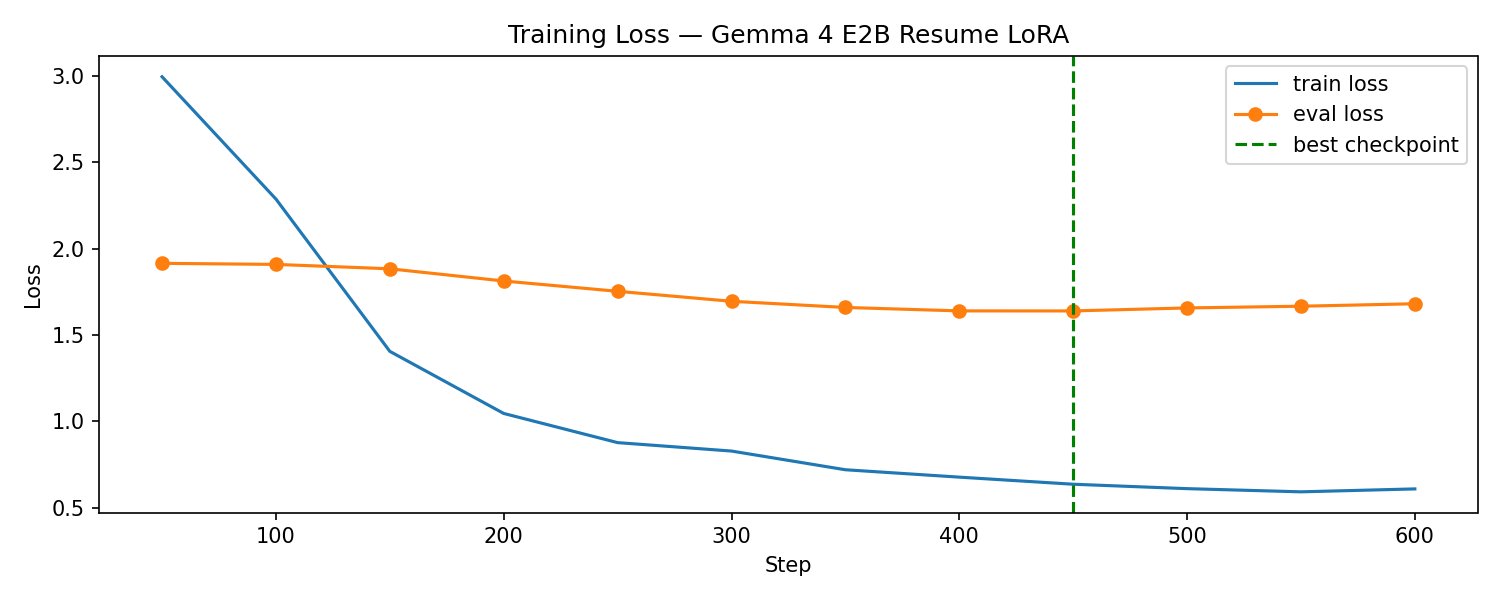
\includegraphics[width=\linewidth]{figures/training_loss.png}
\end{column}
\begin{column}{0.40\textwidth}
  \small
  \begin{itemize}
    \setlength\itemsep{0.4em}
    \item Both train and val loss decrease steadily
    \item Best checkpoint restored at step 450 (early stopping)
    \item \alert{Persistent train/val gap}: model learned the task but did not fully generalize
    \item Likely causes: label noise, modest dataset size, BF16 train vs.\ Q4 eval mismatch
  \end{itemize}
\end{column}
\end{columns}
\end{frame}

% ===============================================================
\begin{frame}{Results}
\begin{columns}[T]
\begin{column}{0.50\textwidth}
  \small
  \begin{table}
  \caption{Evaluation on 100 held-out examples}
  \centering
  \begin{tabular}{lcc}
    \toprule
    Metric & Base & \textbf{Fine-tuned} \\
    \midrule
    Score agreement ($\pm$10 pts) & 49\% & \highlight{75\%} \\
    Experience level accuracy     & 64\% & \highlight{87\%} \\
    Match score MAE               & 13.49 & \highlight{9.11} \\
    Over-qualified FP             & 19    & \highlight{2} \\
    \bottomrule
  \end{tabular}
  \end{table}
  \normalsize
  \textbf{+26 pp} score agreement \quad \textbf{+23 pp} classification accuracy
\end{column}
\begin{column}{0.48\textwidth}
  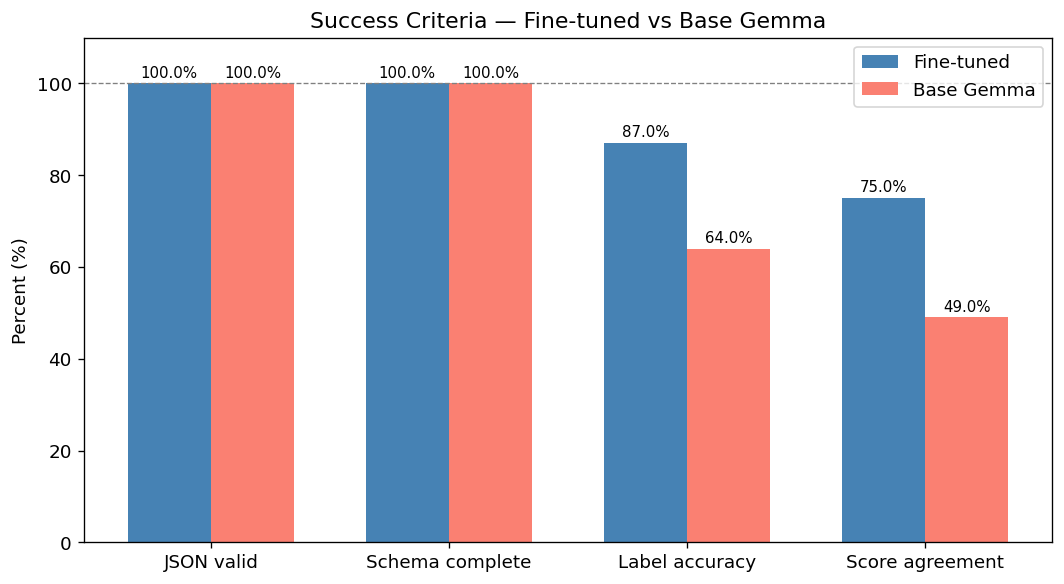
\includegraphics[width=\linewidth]{figures/success_criteria_comparison.png}
\end{column}
\end{columns}
\end{frame}

% ===============================================================
\begin{frame}{Results --- Classification \& Score Error}
\begin{columns}[T]
\begin{column}{0.48\textwidth}
  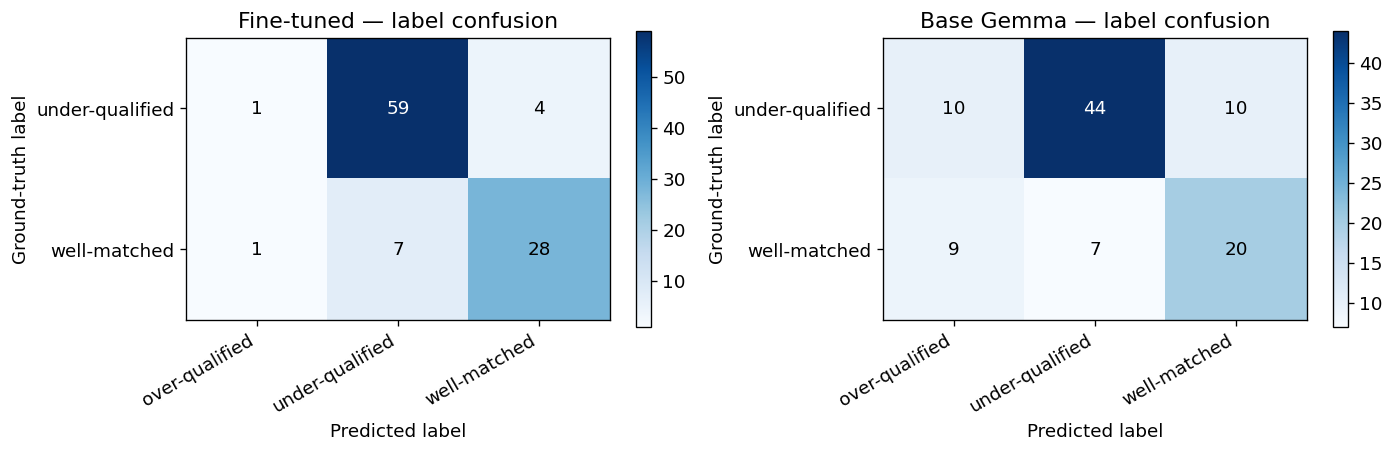
\includegraphics[width=\linewidth]{figures/label_confusion.png}
  \small
  Base model: \alert{19/100 false ``over-qualified''} with \emph{zero} ground-truth over-qualified cases.
  Fine-tuned: reduced to \highlight{2}.
\end{column}
\begin{column}{0.48\textwidth}
  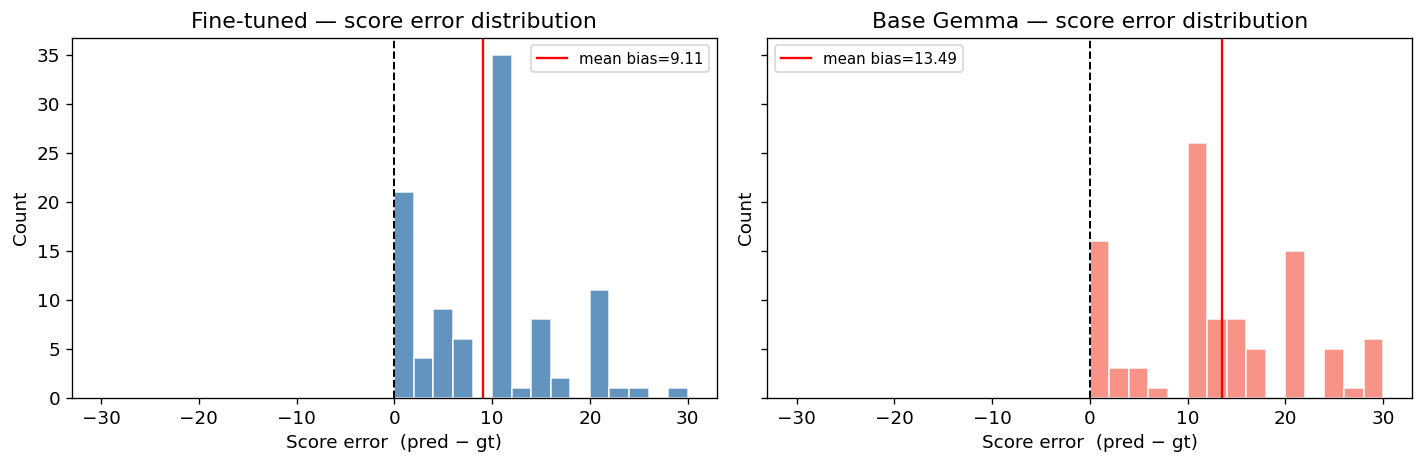
\includegraphics[width=\linewidth]{figures/score_error_histogram.png}
  \small
  Fine-tuned errors cluster near 0; base model spreads to $\pm$30 pts.
  Both models show \alert{consistent positive bias}.
\end{column}
\end{columns}
\end{frame}

% ===============================================================
\begin{frame}{Demo}
\begin{columns}[T]
\begin{column}{0.50\textwidth}
  \small
  \textbf{Streamlit app --- three pages}
  \begin{enumerate}
    \setlength\itemsep{0.2em}
    \item \textbf{Search}: upload resume PDF $\to$ retrieve top matching jobs from ChromaDB
    \item \textbf{Analyze}: select a job $\to$ structured 8-criteria feedback from fine-tuned Gemma
    \item \textbf{History}: review past analyses
  \end{enumerate}
  \textbf{Success case}\\
  Software engineer resume matched to a Senior SWE posting --- model correctly identifies matching skills, gaps, and actionable improvements.
\end{column}
\begin{column}{0.47\textwidth}
  \small
  \textbf{Failure case / limitations}
  \begin{itemize}
    \setlength\itemsep{0.2em}
    \item \alert{Positive scoring bias}: weak matches score 10--15 pts above teacher label
    \item \alert{Short/sparse resumes}: JSON may be missing fields or truncated
    \item \alert{LM Studio must be running}: local server required---no cloud fallback
  \end{itemize}
  \begin{block}{Backup plan}
    \small Pre-recorded screen capture of both cases ready if live demo fails.
  \end{block}
\end{column}
\end{columns}
\end{frame}

% ===============================================================
\begin{frame}{Strengths \& Limitations}
\begin{columns}[T]
\begin{column}{0.48\textwidth}
  \begin{block}{What worked}
    \small
    \begin{itemize}
      \setlength\itemsep{0.2em}
      \item Full end-to-end pipeline: data $\to$ LoRA $\to$ quant $\to$ local deployment
      \item Meaningful gains from \$4.68 of teacher labels
      \item Runs on M1 8 GB RAM --- no cloud budget at inference
      \item Backend-agnostic: swap model without changing UI
    \end{itemize}
  \end{block}
\end{column}
\begin{column}{0.48\textwidth}
  \begin{alertblock}{Limitations \& next steps}
    \small
    \begin{itemize}
      \setlength\itemsep{0.2em}
      \item \textbf{Persistent positive scoring bias} --- both models over-predict
      \item \textbf{Data quantity is the binding constraint} --- 9K examples insufficient for full generalization
      \item \textbf{Quantization mismatch}: trained BF16, evaluated Q4
      \item \textbf{Better data strategy}: synthetic resumes at varying fit levels
    \end{itemize}
  \end{alertblock}
\end{column}
\end{columns}
\end{frame}

% ===============================================================
\begin{frame}{Takeaways}
\begin{columns}[T]
\begin{column}{0.53\textwidth}
  \begin{enumerate}
    \setlength\itemsep{0.5em}
    \item \textbf{Knowledge distillation scales down}:\\
          \$4.68 + 1 hr A100 $\to$ \highlight{+26 pp} over base model
    \item \textbf{Data quantity is king}:\\
          train/val gap confirmed it directly
    \item \textbf{Design for swap-ability}:\\
          configurable backend, no UI changes needed to upgrade
    \item \textbf{Edge deployment is real}:\\
          Q4 quantization makes 5B-param models viable on commodity hardware
  \end{enumerate}
\end{column}
\begin{column}{0.44\textwidth}
  \begin{block}{Core result}
    \centering
    {\small Score agreement}\\[0.2em]
    \highlight{\large 49\% $\to$ 75\%}\\[0.4em]
    {\small Experience level accuracy}\\[0.2em]
    \highlight{\large 64\% $\to$ 87\%}\\[0.3em]
  \end{block}
  \small
  Runs on an Apple M1 with 8 GB RAM.\\
  No API. No cloud. No ongoing cost.
\end{column}
\end{columns}
\vspace{0.3em}
\begin{center}
  \large \textbf{Thank you.} \quad Questions?
\end{center}
\end{frame}

\end{document}
